\documentclass{article}
\usepackage{graphicx} % Required for inserting images
\usepackage{geometry}
\geometry{margin=0.7in}
\usepackage[T1]{fontenc}%
\usepackage[utf8]{inputenc}%
\usepackage{lmodern}%
\usepackage{textcomp}%
\usepackage{lastpage}%
\usepackage{pdflscape}%
\usepackage[table]{xcolor}%
\usepackage{amsmath}%
\usepackage{color}%
\usepackage{multirow}%
\usepackage{longtable}%
\usepackage{xcolor}%
\usepackage{tabularx}%
\usepackage{ltablex}%
%

\title{BACKTESTING REPORT}
\author{Statistical Arbitrage}
\date{03/04/2024}

\begin{document}

\maketitle

\section{Objective and Constraint}

\begin{table}[ht]
\centering
\begin{tabular}{|l|l|}
\hline
Capital Size              & 10B \\ \hline
Return Objective          & Medium \\ \hline
Liquidity needs           & Low \\ \hline
Time Horizon              & Medium \\ \hline
Other Specific Constraint & N/A \\ \hline
\end{tabular}
\label{tab:objective-constraint}
\end{table}

\section{Trading Algorithm}
\begin{table}[ht]
\centering
\begin{tabular}{|l|l|}
\hline
Algorithm Name           & Statistical Arbitrage  \\ \hline
Target Market            & Future and Stock \\ \hline
Decision-making schedule & Daily \\ \hline
\end{tabular}
\label{tab:trading-algo}
\end{table}

\section{Backtesting Assumption}
\begin{table}[ht]
\centering
\begin{tabular}{|l|l|}
\hline
Liquidity                 & Full \\ \hline
Price slippage            & N/A \\ \hline
Market impact             & N/A \\ \hline
Simulated fill price      & N/A \\ \hline
Transaction fee and taxes & .23 point/ .23\% \\ \hline
Sales proceeds advance    &  Yes\\ \hline
\end{tabular}
\label{tab:backtesting-assumption}
\end{table}

\newgeometry{margin=0.18in}%
\begin{landscape}%
\section{Backtesting Performance Evaluation}%
\label{sec:BacktestingPerformanceEvaluation}%

%
\setlength{\tabcolsep}{2pt}%
\begin{center}%
\begin{tabular}{|p{4.0cm}|>{\centering\arraybackslash}p{3.6cm}|>{\centering\arraybackslash}p{3.6cm}|>{\centering\arraybackslash}p{3.6cm}|>{\centering\arraybackslash}p{3.6cm}||>{\centering\arraybackslash}p{3.6cm}|>{\centering\arraybackslash}p{3.6cm}|}%
\hline%
\textbf{Time Period}&\multicolumn{4}{c||}{\textbf{In{-}Sample}}&\multicolumn{2}{c|}{\textbf{Out{-}of{-}Sample}}\\%
\textbf{}
&\multicolumn{4}{c||}{08-2021-12/2023}
&\multicolumn{2}{c|}{01/2024-12/2024}\\%
\hline%
&\multicolumn{2}{>{\centering\arraybackslash}p{7.2cm}|}{\textbf{Initial Parameters}}&\multicolumn{2}{>{\centering\arraybackslash}p{7.2cm}||}{\textbf{Optimal Parameters}}&\multicolumn{2}{>{\centering\arraybackslash}p{7.2cm}|}{\textbf{Optimal Parameters}}\\%
\cline{2%
-%
7}%
\hline%
&\multicolumn{2}{c|}{
% CHANGEME: INCLUDE GRAPHIC OF INITIAL PARAMETER OF IN-SAMPLE BACKTESTING HERE
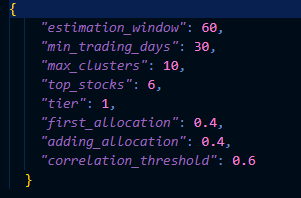
\includegraphics[scale=0.43]{insample_param.png}
}
&\multicolumn{2}{c||}{
% CHANGEME: INCLUDE GRAPHIC OF OPTIMAL PARAMETER OF IN-SAMPLE BACKTESTING HERE
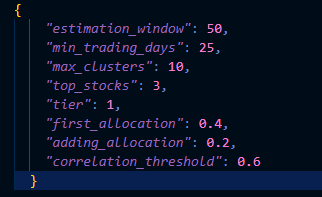
\includegraphics[scale=0.43]{optim_param.png}
}
&\multicolumn{2}{c|}{
% CHANGEME: INCLUDE GRAPHIC OF OPTIMAL PARAMETER OF OUT-OF-SAMPLE BACKTESTING HERE}
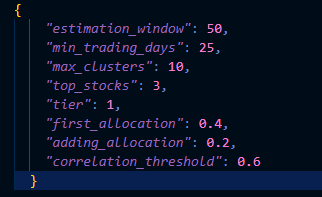
\includegraphics[scale=0.43]{optim_param.png}
}\\%
&\multicolumn{2}{c|}{}&\multicolumn{2}{c||}{}&\multicolumn{2}{c|}{}\\%
&\multicolumn{2}{c|}{
    % CHANGEME: INCLUDE THE DETAILS IN THIS TABLE
    \begin{tabular}{|c|c|c|c|}%
    \hline%
    YEAR & 2021 & 2022 & 2023\\%
    \hline%
    \rowcolor{white}%
    YEARLY & 4.2\% & -25.11\% & -0.12\%\\%
    \hline%
    \rowcolor{lightgray}%
    JAN & n.a\% & -1.27\% & 0.23\%\\%
    \hline%
    \rowcolor{white}%
    FEB & n.a\% & -1.02\% & -2.53\%\\%
    \hline%
    \rowcolor{lightgray}%
    MAR & n.a\% & -3.31\% & 2.90\%\\%
    \hline%
    \rowcolor{white}%
    APR & n.a\% & -6.48\% & -0.11\%\\%
    \hline%
    \rowcolor{lightgray}%
    MAY & n.a\% & -6.66\% & 2.89\%\\%
    \hline%
    \rowcolor{white}%
    JUN & n.a\% & -0.57\% & -0.0\%\\%
    \hline%
    \rowcolor{lightgray}%
    JUL & n.a\% & 0.77\% & -0.07\%\\%
    \hline%
    \rowcolor{white}%
    AUG & 0.00\% & -0.00\% & 0.00\%\\%
    \hline%
    \rowcolor{lightgray}%
    SEP & 0.36\% & -4.47\% & -4.55\%\\%
    \hline%
    \rowcolor{white}%
    OCT & 1.28\% & -5.13\% & -5.32\%\\%
    \hline%
    \rowcolor{lightgray}%
    NOV & 1.55\% & 0.00\% & 5.42\%\\%
    \hline%
    \rowcolor{white}%
    DEC & -0.96\% & 0.00\% & 1.54\%\\%
    \hline%
    \end{tabular}
}
&\multicolumn{2}{c|}{
    % CHANGEME: INCLUDE THE DETAILS IN THIS TABLE
    \begin{tabular}{|c|c|c|c|}%
    \hline%
    YEAR & 2021 & 2022 & 2023\\%
    \hline%
    \rowcolor{white}%
    YEARLY & -2.2\% & -4.4\% & 5.05\%\\%
    \hline%
    \rowcolor{lightgray}%
    JAN & n.a\% & -0.63\% & 3.36\%\\%
    \hline%
    \rowcolor{white}%
    FEB & n.a\% & 1.33\% & -0.27\%\\%
    \hline%
    \rowcolor{lightgray}%
    MAR & n.a\% & 1.64\% & 3.02\%\\%
    \hline%
    \rowcolor{white}%
    APR & n.a\% & -4.04\% & -1.53\%\\%
    \hline%
    \rowcolor{lightgray}%
    MAY & n.a\% & -0.2\% & -0.2\%\\%
    \hline%
    \rowcolor{white}%
    JUN & n.a\% & 3.29\% & 2.27\%\\%
    \hline%
    \rowcolor{lightgray}%
    JUL & n.a\% & 0.35\% & 0.38\%\\%
    \hline%
    \rowcolor{white}%
    AUG & -3.03\% & -0.00\% & 1.14\%\\%
    \hline%
    \rowcolor{lightgray}%
    SEP & -0.28\% & -3.58\% & -3.19\%\\%
    \hline%
    \rowcolor{white}%
    OCT & 1.14\% & -2.41\% & 0.00\%\\%
    \hline%
    \rowcolor{lightgray}%
    NOV & 0.00\% & 0.00\% & -0.31\%\\%
    \hline%
    \rowcolor{white}%
    DEC & 0.00\% & 0.00\% & 0.47\%\\%
    \hline%
    \end{tabular}
}
&\multicolumn{2}{c|}{
    % CHANGEME: INCLUDE THE DETAILS IN THIS TABLE    
    \begin{tabular}{|c|c|c|}%
    \hline%
    YEAR & 2023 & 2024\\%
    \hline%
    \rowcolor{white}%
    YEARLY & 0.00\% &  15.31\%\\%
    \hline%
    \rowcolor{lightgray}%
    JAN & 0.00\% &  3.81\%\\%
    \hline%
    \rowcolor{white}%
    FEB & 0.00\% &  9.68\%\\%
    \hline%
    \rowcolor{lightgray}%
    MAR & 0.00\% &  2.11\%\\%
    \hline%
    \rowcolor{white}%
    APR & 0.00\% &  -1.14\%\\%
    \hline%
    \rowcolor{lightgray}%
    MAY & 0.00\% &  0.00\%\\%
    \hline%
    \rowcolor{white}%
    JUN & 0.00\% &  -0.29\%\\%
    \hline%
    \rowcolor{lightgray}%
    JUL & 0.00\% &  0.38\%\\%
    \hline%
    \rowcolor{white}%
    AUG & 0.00\% &  0.16\%\\%
    \hline%
    \rowcolor{lightgray}%
    SEP & 0.00\% &  2.17\%\\%
    \hline%
    \rowcolor{white}%
    OCT & 0.00\% &  -1.52\%\\%
    \hline%
    \rowcolor{lightgray}%
    NOV & 0.00\% &  -1.16\%\\%
    \hline%
    \rowcolor{white}%
    DEC & 0.00\% &  0.63\%\\%
    \hline%
    \end{tabular}
}\\%
&\multicolumn{2}{c|}{}&\multicolumn{2}{c||}{}&\multicolumn{2}{c|}{}\\%
\hline%
\end{tabular}%
\end{center}%
\begin{center}%
\begin{tabular}{|p{4.0cm}|>{\centering\arraybackslash}p{3.6cm}|>{\centering\arraybackslash}p{3.6cm}|>{\centering\arraybackslash}p{3.6cm}|>{\centering\arraybackslash}p{3.6cm}||>{\centering\arraybackslash}p{3.6cm}|>{\centering\arraybackslash}p{3.6cm}|}%
\hline%
\textbf{Time Period}&\multicolumn{4}{c||}{\textbf{In{-}Sample}}&\multicolumn{2}{c|}{\textbf{Out{-}of{-}Sample}}\\%
\textbf{}
&\multicolumn{4}{c||}{< 08/2022-12/2023>}
&\multicolumn{2}{c|}{<01/2024-12/2024>}\\%
\hline%
&\multicolumn{2}{>{\centering\arraybackslash}p{7.2cm}|}{\textbf{Initial Parameters}}&\multicolumn{2}{>{\centering\arraybackslash}p{7.2cm}||}{\textbf{Optimal Parameters}}&\multicolumn{2}{>{\centering\arraybackslash}p{7.2cm}|}{\textbf{Optimal Parameters}}\\%
\cline{2%
-%
7}%
\hline%
& Portfolio & \multicolumn{2}{>{\centering\arraybackslash}p{7.2cm}|}{VN30} & Portfolio & Portfolio & VN30\\%
\hline%
Beta & 0.24 & \multicolumn{2}{>{\centering\arraybackslash}p{7.2cm}|}{n.a} & 0.12 & 0.22 & n.a\%\\%
\hline%
HPR & -22.05\% & \multicolumn{2}{>{\centering\arraybackslash}p{7.2cm}|}{-20.80\%} & -1.78\% & -1.77\% & 15.31\%\\%
\hline%
Excess HPR & -1.25\% & \multicolumn{2}{>{\centering\arraybackslash}p{7.2cm}|}{n/a} & 22.51\% & -3.52\% & n/a\\%
\hline%
Annual Return & -10.15\% & \multicolumn{2}{>{\centering\arraybackslash}p{7.2cm}|}{-4.24\%} & -0.75\% & -15.37\% & 18.9\%\\%
\hline%
Annual Excess Return & -0.62\% & \multicolumn{2}{>{\centering\arraybackslash}p{7.2cm}|}{n/a} & 10.26\% & -3.54\% & n/a\\%
\hline%
Maximum Drawdown & 30.27\% & \multicolumn{2}{>{\centering\arraybackslash}p{7.2cm}|}{42.46\%} & 8.1\% & 4.32\% & 8.38\%\\%
\hline%
Longest Drawdown & 468 & \multicolumn{2}{>{\centering\arraybackslash}p{7.2cm}|}{472} & 422 & 116 & 71\\%
\hline%
Turnover Ratio & 6.35\% & \multicolumn{2}{>{\centering\arraybackslash}p{7.2cm}|}{n/a} & 7.53\% & 10.87\% & n/a\\%
\hline%
Sharpe Ratio & -1.53 &\multicolumn{2}{>{\centering\arraybackslash}p{7.2cm}|}{-0.65} & -0.86 & 1.47 & 0.97\\%
\hline%
Sortino Ratio & -0.9 & \multicolumn{2}{>{\centering\arraybackslash}p{7.2cm}|}{-0.54} & -0.11 & 3.28 & 1.67\\%
\hline%
Information Ratio & -0.03 & \multicolumn{2}{>{\centering\arraybackslash}p{7.2cm}|}{n/a} & 0.51 & -0.27 & n/a\\%
\hline%
No. stocks in periods&\multicolumn{6}{c|}{}\\%
\hline%
No. held stocks in periods&\multicolumn{6}{c|}{}\\%
\hline%
Excess returns in periods&\multicolumn{6}{c|}{}\\%
\hline%
\end{tabular}%
\end{center}%
\pagebreak%
\end{landscape}
\end{document}
